\documentclass[11pt]{scrartcl}
\usepackage{polski}
\usepackage[polish]{babel}

\usepackage{graphicx, float, caption, subcaption, amsmath}
\usepackage{tabularx, multirow, hyperref, enumitem, listings}
%\usepackage{minted}

\usepackage{listings, xcolor}
\definecolor{md-black}{rgb}{0.12, 0.12, 0.12}
\definecolor{md-teal}{rgb}{0.38, 0.79, 0.69}
\definecolor{md-mauve}{rgb}{0.76, 0.52, 0.75}
\definecolor{md-green}{rgb}{0.13, 0.55, 0.13}
\definecolor{md-red}{rgb}{0.82, 0.10, 0.14}
\definecolor{md-purple}{rgb}{0.69, 0.33, 0.73}
\definecolor{md-orange}{rgb}{0.96, 0.42, 0.18}
\definecolor{md-gray}{rgb}{0.44, 0.46, 0.51}

\lstset{
    language=Python,
    basicstyle=\color{md-teal}\ttfamily,
    keywordstyle=\color{md-mauve},
    commentstyle=\color{md-green},
    stringstyle=\color{md-red},
    numbers=left,
    numberstyle=\small\color{md-gray}\ttfamily,
    stepnumber=1,
    numbersep=5pt,
    backgroundcolor=\color{md-black},
    showspaces=false,
    showstringspaces=false,
    showtabs=false,
    frame=none,
    tabsize=4,
    captionpos=b,
    breaklines=true,
    breakatwhitespace=false,
    escapeinside={\%*}{*)},
    numbersep=-10pt,
    morekeywords={as}
}

\graphicspath{{images/}}

\title{Laboratorium 2 - Regresja liniowa metodą najmniejszych kwadratów}
\author{Mateusz Podmokły - II rok Informatyka WI}
\date{7 marzec 2024}

\begin{document}
    \maketitle

    \section{Treść zadania}
    \textbf{Zadanie 1.} Celem zadania jest zastosowanie metody najmniejszych kwadratów
    do predykcji, czy nowotwór jest złosliwy, czy łagodny. Nowotwory złosliwe i łagodne
    maja rózne charakterystyki wzrostu. \\
    Do rozwiazania problemu wykorzystamy bibliotekę \texttt{pandas}, typ
    \texttt{DataFrame} oraz dwa zbiory danych:
    \begin{itemize}[label=--]
        \item \texttt{breast-cancer-train.dat}
        \item \texttt{breast-cancer-validate.dat}
    \end{itemize}
    Zawierają one klasę nowotworu oraz cechy, tj. charakterystyki nowotworu. \\
    Wykorzystamy liniową oraz kwadratową metodę najmniejszych kwadratów. Dla
    reprezentacji kwadratowej użyjemy tylko podzbioru dostępnych danych, tj.
    danych z kolumn \texttt{radius (mean)}, \texttt{perimeter (mean)},
    \texttt{area (mean)}, \texttt{symetry (mean)}. Do reprezentacji liniowej
    danych metody najmniejszych kwadratów wykorzystamy macierz
    \[
        A_{lin}=
        \begin{bmatrix}
            f_{1,1} & \cdots & f_{1,m} \\
            f_{2,1} & \cdots & f_{2,m} \\
            \vdots & \cdots  & \vdots \\
            f_{n,1} & \cdots & f_{n,m}
        \end{bmatrix}
    \]
    Reprezentacja kwadratowa:
    \[
        A_{quad}=
    \]
    \[
        \begin{bmatrix}
            f_{1,1}, f_{1,2}, f_{1,3}, f_{1,4},
            f_{1,1}^2, f_{1,2}^2, f_{1,3}^2, f_{1,4}^2,
            f_{1_1}f_{1_2}, f_{1_1}f_{1_3}, f_{1_1}f_{1_4},
            f_{1_2}f_{1_3}, f_{1_2}f_{1_4}, f_{1_3}f_{1_4} \\
            \vdots \\
            f_{n,1}, f_{n,2}, f_{n,3}, f_{n,4},
            f_{n,1}^2, f_{n,2}^2, f_{n,3}^2, f_{n,4}^2,
            f_{n_1}f_{n_2}, f_{n_1}f_{n_3}, f_{n_1}f_{n_4},
            f_{n_2}f_{n_3}, f_{n_2}f_{n_4}, f_{n_3}f_{n_4}
        \end{bmatrix}
    \]

    \subsection*{}
    Wagi możemy obliczyć z równania normalnego:
    \[
        w=(A^TA)^{-1}A^Tb
    \]
    Rozwiazujac równanie normalne nalezy uzyc funkcji \texttt{solve} unikając
    obliczania odwrotności macierzy.

    \section{Specyfikacja użytego środowiska}
    Specyfikacja:

    \begin{itemize}
        \item Środowisko: Visual Studio Code,
        \item Język programowania: Python,
        \item System operacyjny: Microsoft Windows 11,
        \item Architektura systemu: x64.
    \end{itemize}

    \section{Rozwiązanie problemu}
    W realizacji rozwiązania wykorzystane zostały następujące biblioteki:

    \begin{lstlisting}
        import pandas as pd
        import numpy as np
        import matplotlib.pyplot as plt
    \end{lstlisting}

    \subsection*{}
    Stworzone zostały reprezentacje danych zawartych w obu zbiorach dla liniowej
    i kwadratowej metody najmniejszych kwadratów (łącznie 4 macierze). Następnie
    stworzony został wektor $b$ dla obu zbiorów, który reprezentuje rodzaj
    nowotworu (1 - złośliwy, -1 - łagodny). \\
    Wagi zostały obliczone w następujący sposób:
    \[
        \texttt{np.linalg.solve}(A^TA,A^Tb)
    \]
    Obliczanie współczynników uwarunkowania macierzy:
    \[
        \texttt{np.linalg.cond}(A^TA)
    \]
    Można sprawdzić skuteczność przewidywań otrzymanych wag. W tym celu
    obliczamy wektor $p$ przez pomnożenie reprezentacji zbiorów walidacyjnych
    z odpowiednimi wektorami wag. Jeżeli $p[i] > 0$, to przewidujemy, że $i$-ta
    osoba ma nowotwór złośliwy, natomiast jeśli $p[i] \leq 0$, to przewidujemy,
    że ma łagodny. Porównane zostały wektory $p$ dla obu reprezentacji
    z odpowiednimi wektorami $b$ w celu wekryfikacji poprawności.

    \section{Przedstawienie wyników}
    \begin{figure}[H]
        \centering
        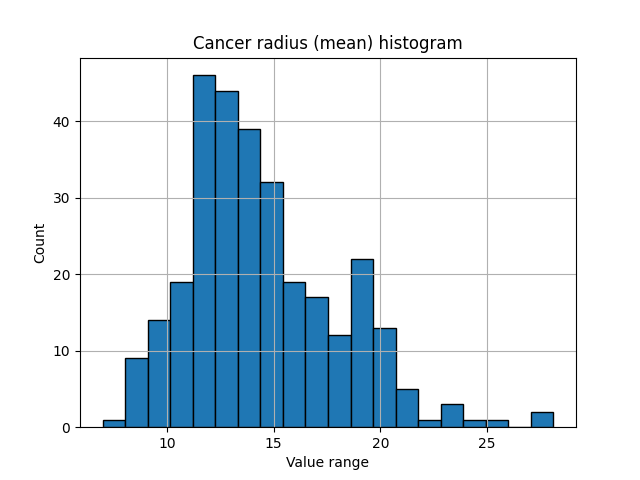
\includegraphics[width=0.8\linewidth]{cancer_radius_hist.png}
        \caption{Histogram przedstawiający średni promień nowotworu.}
    \end{figure}

    Współczynniki uwarunkowania macierzy:
    \[
        cond_{lin} \approx 1.81 \cdot 10^{12}
    \]
    \[
        cond_{quad} \approx 9.06 \cdot 10^{17}
    \]
    Zatem lepiej uwarunkowana jest macierz w przypadku metody liniowej.

    \subsubsection*{Metoda liniowa}
    Prawidłowe rozpoznania nowotworu złośliwego : $58/60$. \\
    Prawidłowe rozpoznania nowotworu łagodnego : $194/200$. \\
    Dokładność: $96.92\%$
    \subsubsection*{Metoda kwadratowa}
    Prawidłowe rozpoznania nowotworu złośliwego : $55/60$. \\
    Prawidłowe rozpoznania nowotworu łagodnego : $185/200$. \\
    Dokładność: $92.31\%$
    \subsubsection*{}
    Wyższą dokładnością charakteryzuje się metoda liniowa.

    \section{Wnioski}

\end{document}
